% interactcadsample.tex
% v1.03 - April 2017

\documentclass[]{interact}

\usepackage{epstopdf}% To incorporate .eps illustrations using PDFLaTeX, etc.
\usepackage{subfigure}% Support for small, `sub' figures and tables
%\usepackage[nolists,tablesfirst]{endfloat}% To `separate' figures and tables from text if required

\usepackage{natbib}% Citation support using natbib.sty
\bibpunct[, ]{(}{)}{;}{a}{}{,}% Citation support using natbib.sty
\renewcommand\bibfont{\fontsize{10}{12}\selectfont}% Bibliography support using natbib.sty

\theoremstyle{plain}% Theorem-like structures provided by amsthm.sty
\newtheorem{theorem}{Theorem}[section]
\newtheorem{lemma}[theorem]{Lemma}
\newtheorem{corollary}[theorem]{Corollary}
\newtheorem{proposition}[theorem]{Proposition}

\theoremstyle{definition}
\newtheorem{definition}[theorem]{Definition}
\newtheorem{example}[theorem]{Example}

\theoremstyle{remark}
\newtheorem{remark}{Remark}
\newtheorem{notation}{Notation}

% see https://stackoverflow.com/a/47122900


\usepackage{hyperref}
\usepackage[utf8]{inputenc}
\usepackage{dcolumn}
\def\tightlist{}

\begin{document}

\articletype{ARTICLE TEMPLATE}

\title{WFH and broadband speed (title needs rework)}


\author{\name{A. N. Author$^{a}$, John Smith$^{b}$}
\affil{$^{a}$Taylor \& Francis, 4 Park Square, Milton Park, Abingdon, UK; $^{b}$Institut für Informatik, Albert-Ludwigs-Universität, Freiburg, Germany}
}

\thanks{CONTACT A. N. Author. Email: \href{mailto:latex.helpdesk@tandf.co.uk}{\nolinkurl{latex.helpdesk@tandf.co.uk}}, John Smith. Email: \href{mailto:john.smith@uni-freiburg.de}{\nolinkurl{john.smith@uni-freiburg.de}}}

\maketitle

\begin{abstract}
TBC
\end{abstract}

\begin{keywords}
covid; internet; working from home; broadband speed; time-series
clusters
\end{keywords}

\hypertarget{sec:1}{%
\section{Introduction}\label{sec:1}}

During the pandemic, working from home using digital technologies,
whether partially or exclusively, was transformed from a niche means of
accessing work, albeit one that had been on a slow, upward trend, to a
widespread way of life in many countries. The ability to work from home
or telecommute meant millions retained their jobs and, to a varying
extent, maintained productivity during periods of strict lockdowns
around the world. However, this ability has not been evenly distributed
socially or spatially, creating a new type of digital divide. On one
side are those who can work from home, supported by digital
technologies, and have thus been able to enjoy both economic resilience
and greater personal safety. On the other side, previously employed
individuals have been forced to accept furlough or redundancy packages
unless they are part of the cadre of essential workers, who are
potentially at high risk of infection. Whilst the basis for this new
digital divide has been viewed as mainly occupational, here we consider
whether the divide is also technological.

Using the UK as a case study, this paper aims to understand how the
quality and reliability of internet service, as reflected in
\emph{experienced} internet speeds, may reinforce or redress the spatial
and social dimensions of the digital division exposed by the pandemic.
To do so, we employ volunteered geographic data on individual broadband
speed tests and state-of-the-art time-series clustering methods to
create clusters of UK local authorities with similar temporal signatures
of experienced internet speeds. We then associate these clusters of
local authorities with their socioeconomic and geographic
characteristics to explore how they overlap with or diverge from the
existing economic and digital geography of the UK. Our analysis enables
us to better understand how the spatial and social distribution of both
occupations and online accessibility intersect to enable or hinder the
practice of telecommuting at a time of extreme demand. We will also
consider what lessons can be learned from this time for a future where
telecommuting is likely to remain a more common means of accessing work,
at least in comparison to the pre-Covid era, and broadband services and
infrastructure must be fit for purpose. \textbf{LET'S LEAVE IT FOR NOW,
BUT I THINK WE CAN CRYSTALISE MORE THE RQ}

The capability to work from home has previously been studied from the
perspective of whether work tasks in a given occupation both can be and
are allowed to be performed using digital technologies independently of
location or co-location with colleagues, including supervisors
\citep{allen2015effective, singh2013modeling}. However, successful
telecommuting also requires that the quality and reliability of digital
services, particularly home internet connection speeds, enable the
completion of work tasks with a minimum of delay or interruption. Prior
to the pandemic, the performance of broadband services with respect to
telecommuters was never tested at scale, as working from home and
connecting to colleagues and workplace resources via the internet was
the purview of a small minority of workers. Instead, leisure use in the
evening, when video streaming services are at their peak, has been used
to benchmark broadband performance and service delivery by different
Internet Service Providers (ISPs), at least in the UK \citep{ofcom2017}.
Yet the shift towards telecommuting during various stages of lockdown
around the world has been drastic and there are speculations that
post-Covid, the tendency to work from home will be much higher than
pre-Covid, raising questions around whether internet services can
accommodate the increased demand. For example, \(47\)\% of people in
employment in the UK worked soley from home in April \(2020\), whilst
the same figure only reached \(5\)\% the year before
\citep{ons2020, ons2020lm2019}. A back of the envelope calculation
suggests that up to 40\% of the working force could work from home on an
ongoing basis \citep{batty2020editorial}. Similar figures have been
reported for other countries \citep{felstead2020homeworking}. For
instance, \(37\)\% of the European workforce worked from home in April
\(2020\) with countries like Finland reaching \(60\)\%
\citep{eurofound2020}. In the US, almost half of the working population
worked from home during the same period because of the pandemic
\citep{brynjolfsson2020covid}, and a recent estimate indicated that
\(37\)\% of all jobs in the US can be permanently performed entirely
from home \citep{NBERw26948}.

None of these changes could have happened in the absence of reliable
information and communication technology (ICT) infrastructure -- both in
terms of software and hardware. But while software innovations are
easily diffused across space and society\footnote{See for example the
  huge success of videoconferencing apps such as Zoom
  \citep{marks2020zoom}.}, the same does not apply for ICT hardware
infrastructure such as internet broadband connectivity. The literature
describes first level digital divides in terms of the availability and
quality of internet connectivity, such as that manifest in different
geographies in the UK
\citep{riddlesden2014broadband, philip2017digital}. Second level digital
divides consider the presence or lack of the necessary skills to
effectively utilise digital technologies and the internet
\citep{blank2014dimensions, van2011internet}. The third level focuses on
the heterogenous returns of internet usage among different socioeconomic
groups and, consequently, how digital technologies can assist in
bridging or further enhancing existing socioeconomic divides.
\citep{stern2009levels, van2014digital, van2015third}. The capability to
telecommute is related to all three levels of digital divides, but more
importantly leads to differentiated outcomes regarding the economic
resilience of people and places to overcome a systemic shock such as the
current pandemic. We identify this as a new digital divide, one that
fundamentally alters the potential returns of internet use for the user
and wider community, assumes skills or functions that are present in
some occupations but not in others, and relies upon access to high
quality internet services. \textbf{WE NEED TO CONNECT OUR FINDINGS WITH
THIS AND JUSTIFY THAT THIS IS INDEED A NEW DIVIDE} As the quality of
internet infrastructure and services, as well as variation in
occupations are spatially dependent and clustered in space, our approach
offers a framework for understanding which types of places, are more
likely to land on the right side of this new digital divide. By asking
how resilient broadband speeds are as experienced in different parts of
the UK during a time of extreme demand, we interrogate which places
benefit from the greater economic resilience digital technologies can
offer, not only during the pandemic, but also into the future.

The structure of this paper is as follows. First we review the
literature on telecommuting and digital divides to better understand the
origins of the new digital divide revealed by the pandemic and its
impact on the economic resilience of different places. We then describe
our data and methodology. Our results section first offers a
classification of how internet services vary across the UK local
authorities and then assesses whether these clusters replicate or
repudiate other socio-economic and geographic patterns of economic
resilience.

\hypertarget{sec:2}{%
\section{Literature review}\label{sec:2}}

\hypertarget{sec:2.1}{%
\subsection{From telecommuting to \#WFH}\label{sec:2.1}}

In this analysis, the terms `telecommuting' and `working from home' are
used interchangeably, as most remote labour during the Covid-19 crisis
was carried out in the homes of individual employees rather than any
other location \citep{eurofound2020}. However, it should be noted that
previous research has explored how telecommuting can occur in other
places, including satellite offices or on public transport
\citep{felstead2012rapid, siha2006telecommuting}. Previous research has
also used a variety of definitions to measure the level of telecommuting
within different workforces, distinguishing, for example, between those
directly employed, indirectly employed, self-employed, full-time or
part-time, and those who use digital technologies to work remotely
full-days or part-days
\citep{allen2015effective, bailey2002review, haddad2009examination}. No
matter the definition, the option and capability to telecommute or work
from home has never been equally distributed spatially or
socio-economically any more than different industries and employment
opportunities have. For example, studies from the United States, the
Netherlands, and the UK found that telecommuters are most likely to hold
professional, managerial, and technical occupations where the workforce
is better educated and wealthier, and that there is suppressed demand
among women and part-time workers
\citep{headicar2016move, peters2004employees, singh2013modeling}.
Opportunities for working from home during the current pandemic have
likewise not been equally spread across the workforce.
\citet{NBERw26948} indicated that in the US, managers, educators, as
well as those working in computer-related occupations, finance, and law
can easily work from home, and that occupations with opportunities to
telecommute are associated with higher earnings. This is not the case
for the workforce occupied in more spatially fixed occupations, from
farming, construction and manufacturing to hospitality and care
services. In the US, these occupations tend to be lower-income,
non-white, without a university degree, live in rental accommodation and
lack health insurance \citep{NBERw27085}. Similar trends can be observed
for other countries. For example, \(75\)\% of workers with tertiary
education worked from home in Europe during spring \(2020\), whilst only
\(34\)\% of workers with secondary education and \(14\)\% of those
primary education did so \citep{eurofound2020}.

\hypertarget{sec:2.2}{%
\subsection{Digital divides and economic resilience}\label{sec:2.2}}

Our understanding of telecommuting as a product of enabled occupations
can be described as a manifestation of the third level digital divide,
as those who are able to use digital technologies to work from home
benefit from a high rate of return on their use of the internet in terms
of autonomy, flexibility, and time saved from commuting
\citep{peters2004employees, siha2006telecommuting, singh2013modeling}.
These returns have been even greater during the Covid-19 crisis, when
those with the ability to telecommute also have the ability to maintain
their employment whilst protecting their health. However, the success of
these arrangements has been dependent upon the first level digital
divide, which is associated with access and quality of internet
connectivity at a time of extremely high demand. \citet{SALEMINK2017360}
provides a systematic review of the pre-pandemic, first level digital
divide in infrastructure quality between urban and rural areas in
various advanced economies. Yet whether this variation in infrastructure
quality affects the spatial footprint of telecommuting has not
previously been measured. There are indications that those who purchase
high speed connections consume more data of all sorts and use their
connections for a variety of purposes \citep{hauge2011consumer}, and
that there is a correlation between access to internet services and a
reduction in household transport spend \citep{bris2017ict}. Whether the
implication is more internet use and less travel because of increased
telecommuting, these studies suggest that better internet services
enable households to make savings and efficiencies, an example of the
first level digital divide reinforcing the third level. Yet did the
purchase of high speed connections and increased internet access also
prepare households for long-term home-working, enforced by government
restrictions? The extreme demand during the pandemic provides a new
opportunity to understand how infrastructure accessibility, quality, and
reliability affects telecommuting, particularly in light of the high
volumes of bandwidth-intensive video conferencing required in order to
avoid the face-to-face contact that could increase the spread of
infection. We seek to answer how internet service resilience contributes
to or reduces economic resilience when the latter is dependent upon the
capability to work from home, and thus improve our understanding of this
new digital divide. \textbf{RELATED TO YOUR POINT ABOVE, WE MAY CONCLUDE
THIS IS NOT A NEW DIGITAL DIVIDE, BUT THAT IS STILL ANSWERING A USEFUL
QUESTION - MIGHT END UP REWORDING AS INTERACTION BETWEEN DIGITAL
DIVIDES? ET: OR REINFORCING THE 3RD LEVEL DIGITAL DIVIDE}

The multi-layered digital divides intersect with material divides and
the economic geography of the UK. Following the regional economic
resilience literature, which underlines the differentiated capacity of
cities and regions to escape or recover from economic crises
\citep{martin2012regional, kitsos2018economic}, different places have
different industrial and occupational profiles, and these affect the
aggregated potential capacity of places for telecommuting. Such profiles
are associated with longstanding inequalities in the UK and their
spatial representation as a North-South divide
\citep{martin_north_south}. Various studies have illustrated severe
inequalities between the north and the south part of the UK regarding,
for example, skills and human capital, unemployment, productivity and
prosperity \citep{lee2014grim, mccann2020perceptions, dorling2018peak}.
Some scholars have even argued that the UK suffers some of the highest
level of interregional inequalities in the global north
\citep{gal2018reducing, mccann2016uk}. Not only are all three levels of
digital divides associated to a certain extent with or shaped by the
geography of the UK, but the intersection of the digital and material
divides affects the capacity of places to overcome some of the economic
effects of the Covid-19 pandemic. Importantly, this is the first time
that digital technologies became an essential tool for economic
resilience for such a great part of the population.

\hypertarget{sec:3}{%
\section{Methods and data}\label{sec:3}}

The starting point of our methodological framework is cluster analysis,
which can be defined within the modern machine learning framework as an
unsupervised learning task, partitioning unlabelled observations into
homogeneous groups known as clusters \citep{montero2014tsclust}. The key
idea is that observations within clusters tend to be more similar than
observations between clusters. Clustering is particularly useful for
exploratory studies as it identifies structures within the data
\citep{aghabozorgi2015time}. Therefore, cluster analysis is a widely
used family of techniques in geography
\citep{gordon1977classification, everitt1974cluster}. For instance,
clustering methods are the basis of \emph{geodemographics}, a research
domain which aims to create small area indicators or typologies of
neighbourhoods based on various and sometimes diverse variables
\citep{SINGLETON2009289, harris2005geodemographics}. Clustering
techniques have also been employed to solve \emph{regionalisation}
problems \citep{niesterowicz2016}.

Common characteristics of these studies are the cross-sectional nature
of the data they employ. Indeed, most clustering problems in geography
deal with observations that are fixed in time. However, for this paper
we are interested in internet speeds, which vary over time and,
therefore, create clusters of local authorities in the UK with similar
temporal signatures of experienced internet speeds. Hence, we deviate
from the established geographical clustering tools and employ
time-series clustering methods.

Time-series clustering methods have been developed in order to deal with
clustering problems linked to, for instance, stock or other financial
data, economic, governmental or medical data as well as machine
monitoring
\citep{aggarwal2013time, aggarwal2001surprising, hyndman2015large, WARRENLIAO20051857}.
The main challenge -- and also the difference with cross-sectional
clustering problems -- is data dimensionality given the multiplicity of
data points for every individual object -- local authorities in our case
-- included in the data set. Time-series are dynamic data as the value
of the observations change as a function of time
\citep{aghabozorgi2015time}. This high dimensionality leads to (i)
computational and algorithmic challenges regarding handling these data
and building algorithms to perform clustering over long time-series, and
(ii) open questions regarding the choice of similarity measures in order
to cluster similar times series objects together considering the whole
length of the time-series and overcoming issues around noise, outliers
and shifts \citep{lin2004iterative, aghabozorgi2015time}.

Time-series clustering methods utilising the whole length of time-series
can be grouped in three categories. The first -- model-based approaches
-- is based on recovering the underlying model for each time-series and
then applying clustering algorithms on the model parameters of each
time-series \citep{aghabozorgi2015time}. The main criticism is the
cluster accuracy for nearby clusters \citep{mitsa2010temporal}. The
second approach is based the formation of vectors of features derived
from the original time-series. These new data of reduced dimensionality
are then clustered using conventional clustering algorithms.

For this paper we utilise the third category of time-series clustering
methods known as shape-based approaches. These methods match two sperate
time-series objects based on the similarity of their shapes through the
calculation of distances between the shapes, and are thus better
equipped to capture similarities between short length time-series
\citep{aghabozorgi2015time}. This approach serves best this paper
because (i) we identify clusters of UK local authorities with similar
temporal signatures -- i.e.~shapes -- of experienced internet speeds and
(ii) the length of our time-series is short (see the data discussion in
this section).

Another import element of time-series clustering is the actual
clustering algorithm. Similar to the clustering of cross-sectional data,
we can employ partitioning algorithms, which lead to non-overlapping
clusters, hierarchical clustering, which classifies clusters at
different levels, and fuzzy algorithms, which create overlapping
clusters \citep{sardatime}. Because of the simplicity of the
implementation and the interpretability of the results, we utilise here
partitioning clustering based on the widely used \emph{k-Means}
algorithm. This is an iterative algorithm, which begins with defining
the desired number of clusters \emph{k}. Then each observation is
randomly assigned to a cluster from the \([1,k]\) space. This initial
cluster assignment is followed by iterations in order to minimise the
distance between the centroids of the clusters and the observations
assigned to these clusters \citep{james2013introduction}.

There are a number of differences between the above described
application of \emph{k-Means} for cross-sectional data and its
application for times series data. Instead of creating clusters around
centroids, a common approach is to create clusters around
\emph{medoids}, which are representative time-series objects with a
minimal distance to all other cluster objects \citep{sardatime}. Also,
instead of calculating the Euclidean distance between centroids and data
points, more complex distance measures need to be employed in order to
capture the similarity between a time-series object and a medoid. A
common distance measure for shape-based time-series clustering is
Dynamic Time Warping (DTW). Using its underpinning dynamic programming
algorithm, DTW compares two time-series objects to find the optimum
warping path between them. DTW is widely used in order to overcome
limitations linked to the use of Euclidean distance
\citep{sardatime, berndt1994using, ratanamahatana2004everything}. The
\texttt{R} package \texttt{dtwclust} has been used for the time-series
clustering \citep{dtwclust}.

To assess the quality and reliability of internet across local
authorities in the UK during the time when the population were told to
work from home if at all possible we utilise unique data comprising
individual internet speed tests from Speedchecker Ltd\footnote{\url{https://www.broadbandspeedchecker.co.uk/}}.
This a private company that allows internet users to check their own
broadband upload and download speeds, and stores every speed-check with
timestamp and geolocation information. These data have been used before
to assess digital divides \citep{riddlesden2014broadband} and the impact
of local loop unbundling regulatory processes
\citep{nardotto2015unbundling}. By using volunteered geographic data, we
are able to assess the \emph{experienced} internet speed by users, which
may differ from the \emph{advertised} maximum speeds of Internet Service
Providers (ISPs). We are particularly interested in upload speeds and
the frequency of speed tests over the period from March to May 2020, as
government statements indicate this is when UK workers were told to work
from home if at all possible \textbf{{[}need ref?{]}}. Average upload
speeds are slower than average download speeds, at \(9.3\)Mb/s mean
upload speed for the whole sample during the period of interest,
compared to \(29.6\)Mb/s for download speeds, but they are also less
associated with internet-based, high-demand, leisure activities such as
video streaming. Therefore, upload speeds are more relevant to
work-related activities such as uploading documents or two-way audio,
video, and text-based communication systems. Meanwhile, the frequency of
speed tests was important in identifying the temporal profile which woud
give us most insight into experienced internet service and resilience,
and provide an indication of the volume of experience over particular
units of time.

The first step in the workflow after dropping some outliers following
\citet{riddlesden2014broadband} was to transform the individual,
geolocated and time-stamped tests to more meaningful aggregates both in
terms of space and time. The frequency of testing indicates that whilst
there is an overall trend of increased testing \textbf{or increased
experience of internet service NOT SURE WHAT THIS MEAND} from March to
April and then a slight reduction from April to May, this trend masks
substantial variation by not only the day of the week, but also time of
day, as can be seen in Figure \ref{test2020}. Thus, a daily aggregation
of upload speeds would mask the variation in experience over the course
of each weekday. Furthermore, the importance of this variation is
highlighted by a comparison with the same period in \(2019\), as in
Figure \ref{test2019}, when the volume of testing and thus of experience
of internet service quality was much more tied to the evening leisure
peak and presumably to download speeds. Since the increase in testing
during the working day in \(2020\) is an indication that users have a
greater perception of the variable quality of internet service,
particularly during a new morning peak of testing for service
reliability, we decided to include a measure of hourly variation in our
temporal profiles. However, although this is a large data set
(\(241,088\) individual tests during the working hours of study period),
there are not enough observations for each Local Authority District
(LAD) and for each working hour of each working day (\(631\) speed tests
per LAD on average) to profile speeds at that level of detail.
Therefore, we aggregate all the speed-checks during the \(13\) weeks of
March to May inclusive for weekdays in \(2020\) by each hour of the day
and day of the week. As our research aims to identify the geography of
internet service resilience for work purposes, bank holidays and the
hours between midnight and 6:00 were excluded, as well as weekend days.
The composite week time-series thus comprise \(18\) hours multiplied by
\(5\) weekdays or \(90\) time points per series. We also aggregate these
data spatially because we could not follow individuals or households and
connect data points. The time-series were calculated for each of the
\(382\) LADs in the UK, standardised, and then a \emph{k}-means
partitioning around medoids clustering algorithm was applied using DTW.
We initially run the algorithm for \(k \in \mathbb{N} \bigcap [5,15]\)
and used cluster validity indices (CVIs) to pick the optimal solution of
\(k = 13\). Following \citet{sardatime} the majority vote for the
following CVIs was used: Silhouette (max), Score function (max),
Calinski-Harabasz (max), Davies-Bouldin (min), Modified Davies-Bouldin
(DB*, min), Dunn (max), COP (min).

\begin{figure}
\centering
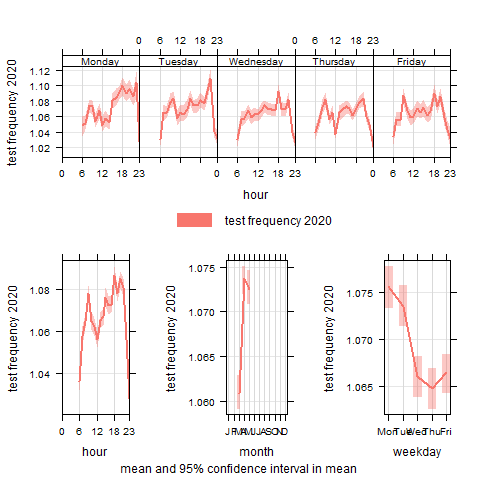
\includegraphics[width=0.75\textwidth,height=0.4\textheight]{figures/time.var.plot2020.png}
\caption{Speed tests over time, 2020 \label{test2020}}
\end{figure}

\begin{figure}
\centering
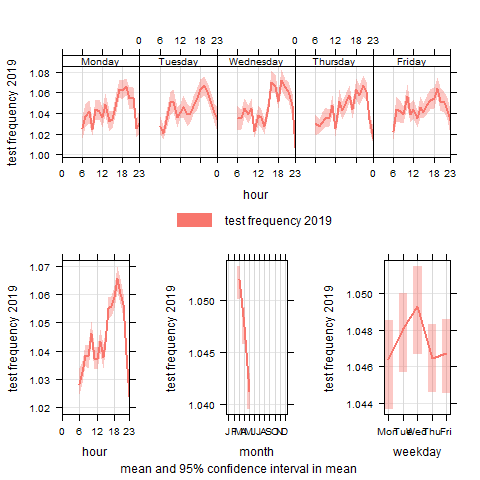
\includegraphics[width=0.75\textwidth,height=0.4\textheight]{figures/time.var.plot2019.png}
\caption{Speed tests over time, 2019 \label{test2019}}
\end{figure}

We then review the characteristics of each cluster, including number of
LADs, and the temporal profile of upload speed by hour of the day and
day of the composite week. Since the quality and reliability of internet
services vary in time and space due to both supply and demand-side
influences, we use a number of different measures to then describe
experienced upload speeds per cluster. These include: a) mean,
experienced connection speed, b) standard deviation or the amount of
fluctuation from the mean, and c) the variation in speeds at particular
times of day when working from home is more likely to take place. We
take account of all three measurements in our descriptives statistics of
upload speeds in order to determine how resilient broadband speeds are
as experienced in different parts of the UK during a time of extreme
demand.

\textbf{More data details and some figures, descriptive stats}

The cause of these different experiences of broadband resilience may be
different in different areas, as they may reflect either similarities in
patterns of demand or similar quality of infrastructure. Our approach is
also limited by potential endogeneity, as for example, better quality
connections with high mean speeds may enable more working from home, but
greater demand may cause slower speeds, less reliability and greater
variability of speed at different times of day or week. Therefore, we
avoid attributing any cause to our analysis of the experienced level of
quality and reliability of upload speeds. Instead, we run an auxiliary
regression in order to understand how the spatial and temporal patterns
of internet service relate to the economic geography of the UK. We
discuss how the different patterns might support or undermine efforts to
work from home and maintain safe productivity and whether they reinforce
existing spatial and social inequalities. More specifically, we estimate
the following multinomial model:

\begin{align}
Pr(Y_{i}=j) = \frac{exp^{X_{i}\beta_{j}}}{\sum_{i=1}^j exp^{X_{i}\beta_{j}}}
\begin{cases}
    i = 1, 2, ... , N \\  
    j = 1, 2, ... , J
\end{cases}\label{eq1}
\end{align}

The identification strategy is as follows. Based on the outcomes of the
time-series clustering, we identify \(J\) distinct and crisp clusters.
We then regress this cluster membership against a vector \(X_{i}\) of
socio-economic and geographic variables, which are discussed in detail
in Section \ref{#sec:4.2}. This analysis enables us to provide a more
nuanced understanding of how telecommuting and technology intersect at a
time of extreme demand, and what lessons this time has for a future
where telecommuting is likely to remain a common means of accessing work
and broadband services, as well as infrastructure, must be fit for
purpose.

\hypertarget{sec:4}{%
\section{Results}\label{sec:4}}

\hypertarget{sec:4.1}{%
\subsection{Upload Clusters / cluster description}\label{sec:4.1}}

The temporal profiles of the local authority clusters have been
summarised in Figures \ref{UpClusterL} and \ref{UpClusterS} and Table
\ref{up.cluster.descr}. The graphs show a composite profile of mean
upload speeds per hour per day for each cluster, with the largest, in
terms of the LAD membership, five clusters in Figure \ref{UpClusterL},
and the next six in Figure \ref{UpClusterS}. These figures and table
provide a comprehensive overview of the quality and reliability of
experienced broadband in different parts of the UK, the temporal
clusters offering a novel approach to understanding spatial disparity.

\begin{figure}
\includegraphics[width=0.95\linewidth]{figures/upClusterL} \caption{\label{UpClusterL}Temporal profilies for upload speed large clusters}\label{fig:unnamed-chunk-2}
\end{figure}

\begin{figure}
\includegraphics[width=0.95\linewidth]{figures/upClusterS} \caption{\label{UpClusterS}Temporal profilies for upload speed small clusters}\label{fig:unnamed-chunk-3}
\end{figure}

\begin{table}[!htbp] \centering 
  \caption{Upload speed cluster characteristics\label{up.cluster.descr}} 
  \label{} 
\footnotesize 
\begin{tabular}{@{\extracolsep{0pt}} ccccccc} 
\\[-1.8ex]\hline 
\hline \\[-1.8ex] 
Cluster & N. of LADs & LAD population & mean speed & SD speed & mean AM speed & mean PM speed \\ 
\hline \\[-1.8ex] 
1 & 5 & 343100 & 8557.389 & 6138.998 & 7746.892 & 9562.508 \\ 
2 & 2 & 265600 & 10921.69 & 6686.872 & 9674.043 & 10645.43 \\ 
3 & 4 & 474700 & 10200.753 & 5658.418 & 9470.446 & 11236.237 \\ 
4 & 1 & 91100 & 9688.899 & 6121.587 & 7816.234 & 9689.224 \\ 
5 & 1 & 79800 & 10126.506 & 6024.124 & 9030.22 & 11100.605 \\ 
6 & 155 & 29535700 & 9396.565 & 5839.097 & 9161.33 & 9580.422 \\ 
7 & 4 & 559800 & 10119.495 & 6102.311 & 9813.353 & 11070.093 \\ 
8 & 5 & 436300 & 9428.931 & 6254.047 & 8681.534 & 10434.339 \\ 
9 & 32 & 6355500 & 10878.131 & 5957.156 & 10831.557 & 11070.88 \\ 
10 & 4 & 699600 & 10795.469 & 6005.111 & 9257.855 & 10697.492 \\ 
11 & 33 & 5771400 & 10845.045 & 5936.36 & 10780.877 & 10987.827 \\ 
12 & 10 & 1544900 & 9550.756 & 6165.524 & 9254.436 & 9047.503 \\ 
13 & 126 & 20277700 & 8392.451 & 5849.227 & 8298.513 & 8521.828 \\ 
\hline \\[-1.8ex] 
\multicolumn{7}{l}{Note: All speed measures are upload speeds} \\ 
\end{tabular} 
\end{table}

The largest two clusters, comprising \(281\) local authorities and
almost \(50\) million people, fall into clusters \(6\) and cluster
\(13\). Cluster \(13\) has one of the lowest aggregate mean upload speed
of any of the clusters, and the second highest ratio of the standard
deviation to the mean. This suggests that those living in local
authorities in this cluster experienced some of the lowest quality
broadband services in terms of upload speeds in the UK. However, the
variation in upload speeds in cluster \(13\), which can be an indication
of its reliability, does not seem to disproportionately affect the
morning peak from 9:00-10:59, as upload speeds are, on average, only
\(2.6\)\% slower than in the evening peak period between 19:00 and
20:59. Although cluster \(13\) does include some rural, remote areas of
the country, such as Northwest Scotland, Cornwall and Powys in Wales as
shown on Figure \ref{map.up.clusters}, it also includes the major
metropolitan centres of Bristol, Liverpool, and Newcastle, as well as
nine (of \(32\)) London Boroughs and plenty of home county and suburban
areas. Meanwhile, those living in cluster \(6\) experience aggregate
mean upload speeds of about \(1\)Mb/s faster than those in cluster
\(13\), but still lower than the other three large clusters and most of
the smaller clusters, suggesting a middling quality of service. However,
the time profile for cluster \(6\) in Figure \(3\)a shows that upload
speeds drop quickly from \(6:00\) to 7:00 on a Monday and peak between
23:00 and midnight on Wednesday and Thursday, but tend to be lower
during the working day. Indeed, those in cluster \(6\), including people
living in Birmingham, Leeds and Sheffield, in \(12\) London Boroughs,
and many suburban areas and smaller cities like Cardiff, Oxford and
Cambridge experience mean upload speeds in the morning that are
\(4.4\)\% lower than in the evening. This lower level of reliability may
be as a result of increased demand, e.g.~for telecommuting, especially
as there are few truly remote areas in this cluster.

\begin{figure}
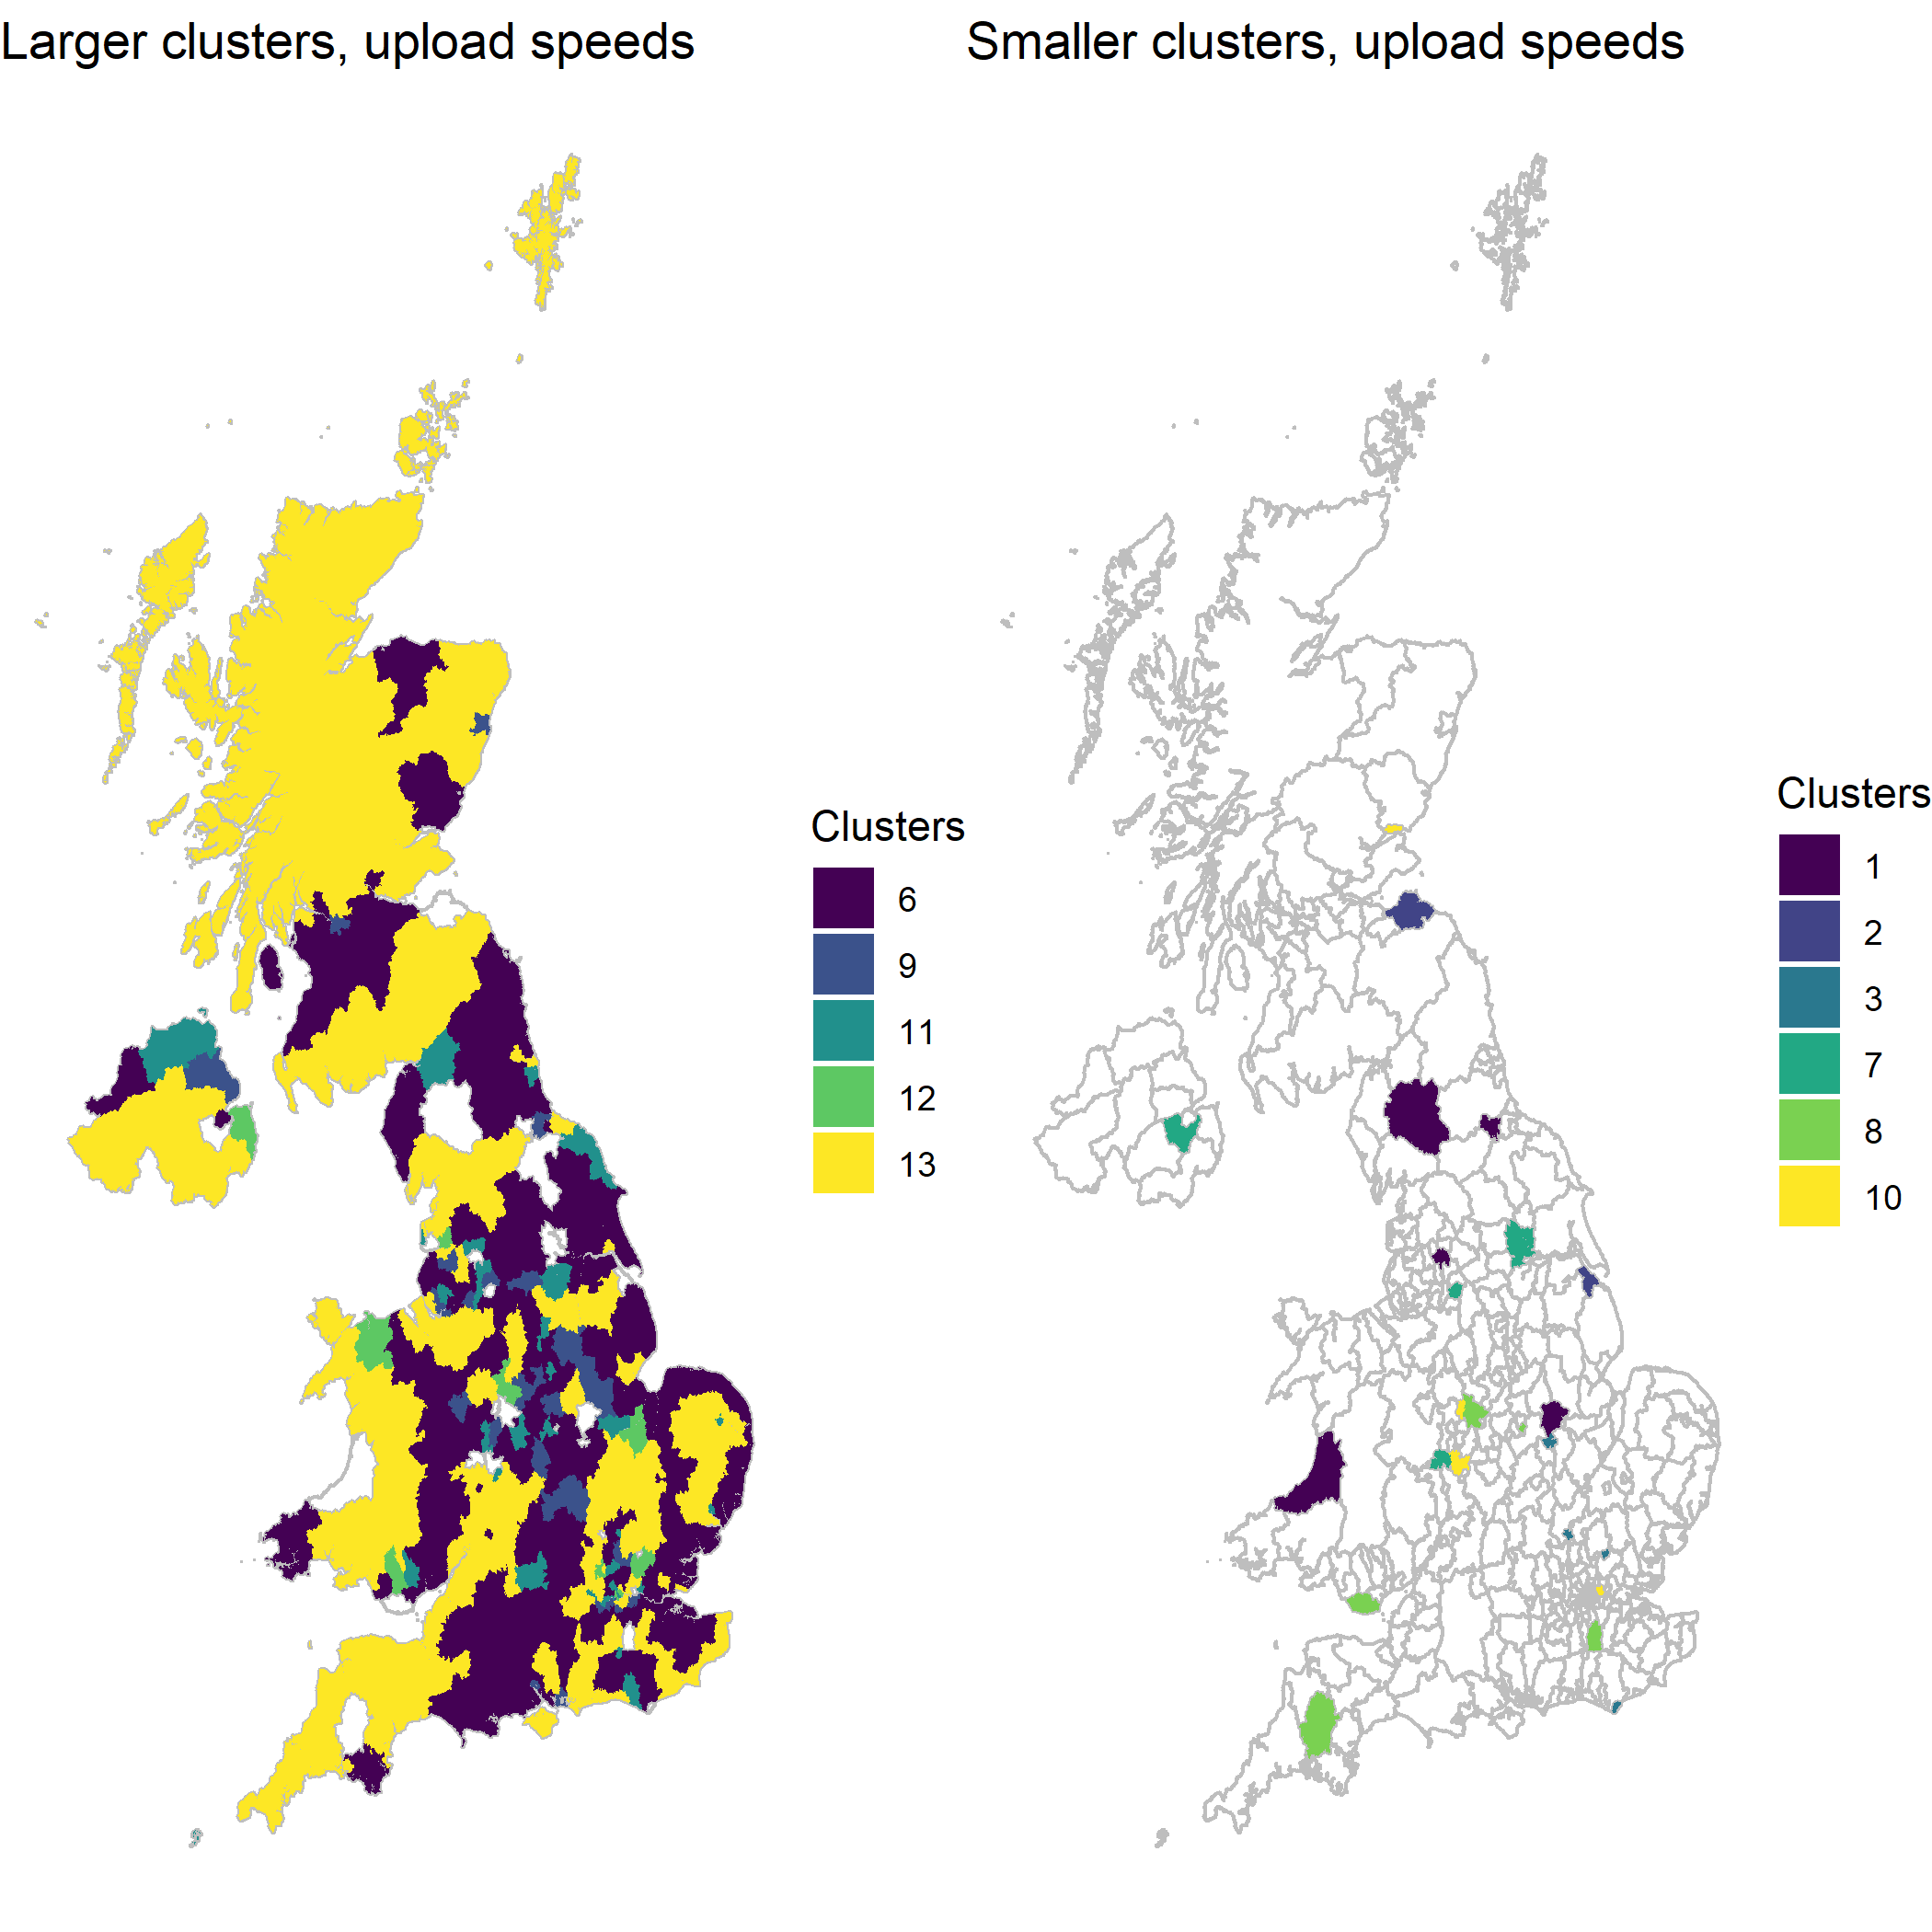
\includegraphics[width=0.95\linewidth]{figures/map.up.clusters} \caption{\label{map.up.clusters}Upload speed clusters for LADs}\label{fig:unnamed-chunk-5}
\end{figure}

However, whilst the difference in experienced mean upload speeds between
9:00-10:59 and 19:00-20:59 in cluster \(6\) is greater than in any of
the other large clusters, it is smaller than this difference in all the
clusters shown in Figure \ref{UpClusterL}. Whilst this may suggest a
lack of reliability, especially considering the large spikes and dips in
these clusters, the statistics in Table \(1\) show a more varied
picture. The experienced upload speeds in cluster \(1\) are the second
slowest of any cluster, the ratio of standard deviation to mean is the
highest, as is the ratio of speeds in the morning compared to the
evening peak hours analysed. The five, mainly rural authorities in this
cluster clearly lack broadband resilience, for telecommuting or
otherwise. Home to almost \(3.5\) thousand people, the districts are
scattered around the country: Ceredigion in West Wales, Darlington in
the Northeast, Eden between the Lake District and the North Penines,
Rossendale in the Northwest, and Rutland in the East Midlands. In
comparison, clusters \(3\) and \(10\) have relatively high mean upload
speeds, and low standard deviations, suggesting reliability and
resilience, as well as quality broadband services, despite slower speeds
in the morning peak. Like cluster \(6\), is this also a sign of
increased telecommuting? The eight LADs in clusters \(3\) and \(10\) are
home to over one million people, and are all more urban and suburban
than cluster \(1\), including the London Borough of Newham, the
Southeast commuter towns of Harlow and Luton, the Birmingham suburbs of
Bromsgrove and Cannock Chase, Dundee City, and the towns of Eastbourne
and Corby.

Meanwhile, the most resilient broadband service in terms of both quality
and reliability appears to be found in clusters \(9\) and \(11\), home
to over \(12\) million people. The mean speeds for these clusters are
second and third highest, the ratio of the standard deviation to the
mean are the two lowest, and the experienced upload speeds in the
morning peak are not that different from those experienced in the
evening peak. In Figure \ref{UpClusterL}, cluster \(11\) shows more
noticeable peaks and troughs, but the lowest points are not at the peak
times described in Table \(1\). Rather, the slowest upload speeds on
average occur between 6:00-7:00 on Monday morning, 14:00-15:00 on
Friday, and \(16:00-17:00\) on Thursday. These slowest times are still
mostly faster than the average hourly upload speeds in cluster \(13\).
Although not all of the local authorities in these two clusters are
urban, among the \(65\) LADs are Manchester and three of the nine other
boroughs of Greater Manchester, Glasgow, Nottingham, both Portsmouth and
Southampton, eight London Boroughs, four of the seven constituent
authorities of the West Midlands Combined Authority. There are also a
number of other tightly bounded urban areas, such as Aberdeen,
Blackpool, Ipswich, Norwich, Slough, and Stevenage, and urban areas at
the centre of less confined districts like Burnley, Milton Keynes, and
Northampton. The local authorities in these two clusters clearly
experienced resilient broadband that could support high levels of
telecommuting. They are \emph{not} on the wrong side of the first level
digital divide, but how likely are they to be able to take advantage of
their resilient ICT infrastructure and services?

\hypertarget{sec:4.2}{%
\subsection{aux regressions}\label{sec:4.2}}

\begin{sidewaystable}[!htbp] \centering 
  \caption{Auxiliary multinomial regression of upload speed clusters on socio-economic and geographic LAD variables\label{aux}} 
  \label{} 
\tiny 
\begin{tabular}{@{\extracolsep{5pt}}lccccccccccc} 
\\[-1.8ex]\hline 
\hline \\[-1.8ex] 
\\[-1.8ex] & 1 & 2 & 3 & 6 & 7 & 8 & 9 & 10 & 11 & 12 & 13 \\ 
\\[-1.8ex] & (1) & (2) & (3) & (4) & (5) & (6) & (7) & (8) & (9) & (10) & (11)\\ 
\hline \\[-1.8ex] 
 pop, 2018 & $-$0.00004$^{***}$ & 0.00002$^{*}$ & 0.00001 & 0.00002$^{***}$ & 0.00002$^{***}$ & 0.00000 & 0.00002$^{***}$ & 0.00002$^{***}$ & 0.00002$^{***}$ & 0.00002$^{**}$ & 0.00002$^{***}$ \\ 
  & (0.00002) & (0.00001) & (0.00001) & (0.00001) & (0.00001) & (0.00002) & (0.00001) & (0.00001) & (0.00001) & (0.00001) & (0.00001) \\ 
  & & & & & & & & & & & \\ 
 job density, 2018 & $-$0.536$^{***}$ & $-$1.834$^{***}$ & $-$0.132$^{***}$ & $-$0.925$^{***}$ & $-$1.208$^{***}$ & $-$0.299$^{***}$ & $-$1.746$^{***}$ & $-$1.436$^{***}$ & 3.350$^{***}$ & 3.400$^{***}$ & 0.630$^{***}$ \\ 
  & (0.00000) & (0.00000) & (0.00000) & (0.00000) & (0.00000) & (0.00000) & (0.00000) & (0.00000) & (0.00000) & (0.00000) & (0.00000) \\ 
  & & & & & & & & & & & \\ 
 distance to nearest met. area & $-$0.034$^{***}$ & $-$0.014$^{***}$ & 0.002$^{***}$ & $-$0.020$^{***}$ & $-$0.074$^{***}$ & $-$0.044$^{***}$ & $-$0.013$^{***}$ & $-$0.036$^{***}$ & $-$0.031$^{***}$ & $-$0.036$^{***}$ & $-$0.024$^{***}$ \\ 
  & (0.0005) & (0.001) & (0.0002) & (0.002) & (0.0001) & (0.0002) & (0.002) & (0.0005) & (0.0003) & (0.0002) & (0.002) \\ 
  & & & & & & & & & & & \\ 
 distance to London & 0.007$^{***}$ & 0.002 & $-$0.016$^{***}$ & 0.001 & 0.004$^{***}$ & 0.004$^{***}$ & $-$0.002$^{*}$ & 0.005$^{**}$ & $-$0.002 & 0.003 & 0.006$^{***}$ \\ 
  & (0.001) & (0.002) & (0.0004) & (0.001) & (0.001) & (0.001) & (0.001) & (0.002) & (0.002) & (0.002) & (0.001) \\ 
  & & & & & & & & & & & \\ 
 South of the UK & $-$0.410$^{***}$ & $-$1.451$^{***}$ & $-$0.039$^{***}$ & $-$0.111$^{***}$ & $-$0.048$^{***}$ & $-$0.841$^{***}$ & $-$0.798$^{***}$ & 1.492$^{***}$ & 0.610$^{***}$ & 0.798$^{***}$ & 2.403$^{***}$ \\ 
  & (0.00000) & (0.00000) & (0.00000) & (0.00001) & (0.00000) & (0.00000) & (0.00001) & (0.00000) & (0.00001) & (0.00001) & (0.00001) \\ 
  & & & & & & & & & & & \\ 
 managerial jobs, 2020 & 0.939$^{***}$ & 0.704$^{***}$ & 0.435$^{***}$ & 0.704$^{***}$ & 0.316$^{***}$ & 0.786$^{***}$ & 0.576$^{***}$ & 0.311$^{***}$ & 0.476$^{***}$ & 0.594$^{***}$ & 0.615$^{***}$ \\ 
  & (0.00004) & (0.0001) & (0.00004) & (0.00004) & (0.00002) & (0.0001) & (0.00003) & (0.00003) & (0.00002) & (0.00004) & (0.00003) \\ 
  & & & & & & & & & & & \\ 
 tech jobs, 2020 & 0.096$^{***}$ & $-$0.257$^{***}$ & $-$0.071$^{***}$ & $-$0.111$^{***}$ & $-$0.206$^{***}$ & 0.199$^{***}$ & $-$0.126$^{***}$ & $-$0.606$^{***}$ & $-$0.180$^{***}$ & $-$0.398$^{***}$ & $-$0.112$^{***}$ \\ 
  & (0.00004) & (0.00004) & (0.00004) & (0.00003) & (0.00003) & (0.0001) & (0.00003) & (0.00003) & (0.00002) & (0.00004) & (0.00003) \\ 
  & & & & & & & & & & & \\ 
 skilled trade jobs, 2020 & 0.651$^{***}$ & 0.160$^{***}$ & $-$0.191$^{***}$ & 0.236$^{***}$ & 0.604$^{***}$ & $-$0.184$^{***}$ & 0.205$^{***}$ & 0.597$^{***}$ & 0.108$^{***}$ & $-$0.022$^{***}$ & 0.295$^{***}$ \\ 
  & (0.00004) & (0.00004) & (0.00003) & (0.00003) & (0.00003) & (0.00004) & (0.00002) & (0.00003) & (0.00003) & (0.00004) & (0.00003) \\ 
  & & & & & & & & & & & \\ 
 professional jobs, 2020 & $-$0.118$^{***}$ & $-$0.234$^{***}$ & $-$0.121$^{***}$ & $-$0.172$^{***}$ & $-$0.514$^{***}$ & $-$0.172$^{***}$ & $-$0.349$^{***}$ & $-$0.351$^{***}$ & $-$0.245$^{***}$ & $-$0.344$^{***}$ & $-$0.229$^{***}$ \\ 
  & (0.00005) & (0.0001) & (0.0001) & (0.00005) & (0.00003) & (0.0001) & (0.00004) & (0.0001) & (0.00003) & (0.00005) & (0.0001) \\ 
  & & & & & & & & & & & \\ 
 administrative jobs, 2020 & 0.019$^{***}$ & $-$0.836$^{***}$ & $-$0.040$^{***}$ & $-$0.117$^{***}$ & $-$0.139$^{***}$ & 0.206$^{***}$ & $-$0.058$^{***}$ & $-$0.200$^{***}$ & $-$0.055$^{***}$ & $-$0.168$^{***}$ & $-$0.177$^{***}$ \\ 
  & (0.00003) & (0.00002) & (0.00004) & (0.00001) & (0.00003) & (0.00003) & (0.00001) & (0.00002) & (0.00002) & (0.00002) & (0.00002) \\ 
  & & & & & & & & & & & \\ 
 leisure jobs, 2020 & $-$0.198$^{***}$ & $-$0.180$^{***}$ & $-$0.225$^{***}$ & $-$0.476$^{***}$ & $-$0.654$^{***}$ & $-$0.820$^{***}$ & $-$0.537$^{***}$ & $-$0.935$^{***}$ & $-$0.353$^{***}$ & $-$0.625$^{***}$ & $-$0.491$^{***}$ \\ 
  & (0.00002) & (0.00004) & (0.00004) & (0.00002) & (0.00002) & (0.00003) & (0.00002) & (0.00001) & (0.00002) & (0.00003) & (0.00002) \\ 
  & & & & & & & & & & & \\ 
 machine operation jobs, 2020 & $-$0.336$^{***}$ & 0.207$^{***}$ & 0.392$^{***}$ & 0.010$^{***}$ & $-$0.433$^{***}$ & 0.139$^{***}$ & $-$0.099$^{***}$ & $-$0.139$^{***}$ & $-$0.144$^{***}$ & 0.098$^{***}$ & $-$0.179$^{***}$ \\ 
  & (0.00002) & (0.00003) & (0.00003) & (0.00002) & (0.00001) & (0.00003) & (0.00002) & (0.00001) & (0.00001) & (0.00002) & (0.00001) \\ 
  & & & & & & & & & & & \\ 
 earnings, 2019 & $-$0.003$^{*}$ & 0.010$^{***}$ & 0.012$^{***}$ & 0.020$^{***}$ & 0.027$^{***}$ & 0.001 & 0.020$^{***}$ & 0.016$^{***}$ & 0.015$^{***}$ & 0.025$^{***}$ & 0.014$^{***}$ \\ 
  & (0.002) & (0.002) & (0.002) & (0.001) & (0.001) & (0.003) & (0.001) & (0.002) & (0.001) & (0.001) & (0.001) \\ 
  & & & & & & & & & & & \\ 
 n. business est. per hab., 2019 & 0.126$^{***}$ & $-$0.120$^{***}$ & $-$0.094$^{***}$ & $-$0.133$^{***}$ & 0.123$^{***}$ & $-$0.051$^{***}$ & $-$0.334$^{***}$ & $-$0.133$^{***}$ & $-$0.150$^{***}$ & 0.289$^{***}$ & 0.377$^{***}$ \\ 
  & (0.00000) & (0.00000) & (0.00000) & (0.00000) & (0.00000) & (0.00000) & (0.00000) & (0.00000) & (0.00000) & (0.00000) & (0.00000) \\ 
  & & & & & & & & & & & \\ 
 NVQ4+ & $-$0.141$^{***}$ & 0.064$^{***}$ & $-$0.091$^{***}$ & $-$0.070$^{***}$ & $-$0.010$^{***}$ & 0.004$^{***}$ & 0.016$^{***}$ & 0.170$^{***}$ & $-$0.110$^{***}$ & $-$0.038$^{***}$ & $-$0.035$^{***}$ \\ 
  & (0.0001) & (0.0001) & (0.0001) & (0.0001) & (0.0001) & (0.0002) & (0.0001) & (0.0001) & (0.0001) & (0.0001) & (0.0001) \\ 
  & & & & & & & & & & & \\ 
 AM tests per hab., 2020 & 0.0005$^{***}$ & $-$0.002$^{***}$ & $-$0.005$^{***}$ & 0.010$^{***}$ & 0.0004$^{***}$ & $-$0.001$^{***}$ & $-$0.002$^{***}$ & $-$0.005$^{***}$ & $-$0.013$^{***}$ & $-$0.001$^{***}$ & 0.016$^{***}$ \\ 
  & (0.000) & (0.000) & (0.000) & (0.000) & (0.000) & (0.000) & (0.000) & (0.000) & (0.000) & (0.000) & (0.000) \\ 
  & & & & & & & & & & & \\ 
 % of Virgin Media connections & $-$0.044$^{***}$ & 1.578$^{***}$ & 1.210$^{***}$ & 0.248$^{***}$ & $-$1.724$^{***}$ & $-$0.242$^{***}$ & 3.109$^{***}$ & $-$0.085$^{***}$ & 1.214$^{***}$ & $-$3.889$^{***}$ & $-$0.745$^{***}$ \\ 
  & (0.00000) & (0.00000) & (0.00000) & (0.00000) & (0.00000) & (0.00000) & (0.00000) & (0.00000) & (0.00000) & (0.00000) & (0.00000) \\ 
  & & & & & & & & & & & \\ 
 Constant & 0.321$^{***}$ & $-$0.436$^{***}$ & 0.199$^{***}$ & $-$2.953$^{***}$ & 0.278$^{***}$ & 0.002$^{***}$ & $-$0.866$^{***}$ & 0.788$^{***}$ & 2.600$^{***}$ & 0.017$^{***}$ & 0.022$^{***}$ \\ 
  & (0.00000) & (0.00000) & (0.00000) & (0.00000) & (0.00000) & (0.00000) & (0.00000) & (0.00000) & (0.00000) & (0.00000) & (0.00000) \\ 
  & & & & & & & & & & & \\ 
\hline \\[-1.8ex] 
McFadden's R squared & 0.338 & 0.338 & 0.338 & 0.338 & 0.338 & 0.338 & 0.338 & 0.338 & 0.338 & 0.338 & 0.338 \\ 
N & 323 & 323 & 323 & 323 & 323 & 323 & 323 & 323 & 323 & 323 & 323 \\ 
Akaike Inf. Crit. & 1,148.027 & 1,148.027 & 1,148.027 & 1,148.027 & 1,148.027 & 1,148.027 & 1,148.027 & 1,148.027 & 1,148.027 & 1,148.027 & 1,148.027 \\ 
\hline 
\hline \\[-1.8ex] 
\textit{Note:}  & \multicolumn{11}{r}{$^{*}$p$<$0.1; $^{**}$p$<$0.05; $^{***}$p$<$0.01} \\ 
\end{tabular} 
\end{sidewaystable}

Clusters \(3\), \(9\), \(10\) and \(11\) seem to benefit most from high
quality and resilient broadband services. The dips in mean upload speeds
in clusters \(6\), \(3\) and \(10\) during the morning peak are
suggestive of more use during the working day, and potentially more
telecommuting. Using auxiliary regressions, we test whether the clusters
that have higher mean speeds and more reliable services are more urban,
more wealthy, and / or more likely to benefit from a choice of high
quality internet services. We also measure which of our clusters are
more likely to have a higher proportion of occupations which enable
telecommuting because of the nature of the work. The results of these
auxiliary regressions are presented in Table \ref{aux}. The dependent
variable is the LAD cluster membership as described in Section
\ref{#sec:3} and equation \ref{eq1} and each column represent a
different cluster. The reference case is cluster \(4\), which includes
the local authority of Hambleton in North Yorkshire, a rural area of
just over ninety thousand people. Mean, experienced upload speeds in
cluster \(4\) are close to both the average speeds for the \(13\)
clusters (\(9.9\)Mb/s) and the pre-clustered average for the whole
sample (\(9.3\)Mb/s). The standard deviation for cluster \(4\) and the
ratio of evening to morning peak speeds are indications of worse
reliability than many of the other clusters. Hence, the results in Table
\ref{aux} should be seens as relative rather than absolute
probabilities.

First, the number of speed tests run per cluster inhabitant between
9:00-10:59 is an indication of satisfaction or at least a lack of
concern over broadband speeds and quality of service. People in clusters
\(3\), \(9\), \(10\) and \(11\) all ran fewer speed tests (at a per
capita basis) at this time of day than people in clusters \(6\) and
\(13\). Those in clusters \(3\), \(9\), \(10\) and \(11\) also benefit
from a higher proportion of fast Virgin cable connections than those in
clusters \(6\) and \(13\). Since services provided by Virgin Media are
only available to \(45\)\% of premises in the UK \citep{ofcom2016},
where the more lucrative ICT market originally attracted the cable TV
provider, this is an indication that people in these clusters are more
likely to live on the right side of the first level,
infrastructure-based digital divide. Another indication is if people in
these clusters are more likely to be closer to London or a metropolitan
area. The broadband speed tests run in the authorities in cluster \(3\)
are more likely to be taking place close to London than those run in any
of the other clusters, a result that makes sense considering two of the
four authorities in cluster \(3\) are the London commuter towns of
Harlow and Luton. However, even though London was also included in the
variable calculating distance to one of the ten major metropolitan areas
in England, or Glasgow or Cardiff, tests run in cluster \(3\) are likely
to be furthest away. \textbf{Did you include London in distMet as well?
- code suggests so} \textbf{Do we need to re-think this variable
(e.g.~remove Cardiff, add Leicester or\ldots)}

\hypertarget{sec:5}{%
\section{Conclusions}\label{sec:5}}

The long-term effects of such drastic changes in telecommuting and
attitudes towards working from home are difficult to predict.
Nevertheless, they span through various aspects of economy and society:
from changes to transportation planning due to altered commuting
patters, to changes in land use and urban planning to accommodate people
who work from home \citep{BUDNITZ2020102713}\textbf{also 2020 Swedish
article from JTG}; and from productivity and innovation changes, to
changes in agglomeration externalities and the attraction of large
cities \citep{econobs} just to name a few. This paper is positioned to
support endeavours in understanding the effects of increased
telecommuting by exposing the spatial and social dimensions of
telecommuting including the resilience of broadband speeds in terms of
both quality and reliability of service, and whether this reinforces or
redresses prior digital divisions. \textbf{took this bit you wrote to
put in the discussion at the end?}

\hypertarget{acknowledgements}{%
\section*{Acknowledgement(s)}\label{acknowledgements}}
\addcontentsline{toc}{section}{Acknowledgement(s)}

An unnumbered section,
e.g.~\texttt{\textbackslash{}section*\{Acknowledgements\}}, may be used
for thanks, etc.~if required and included \emph{in the non-anonymous
version} before any Notes or References.

\hypertarget{funding}{%
\section*{Funding}\label{funding}}
\addcontentsline{toc}{section}{Funding}

An unnumbered section,
e.g.~\texttt{\textbackslash{}section*\{Funding\}}, may be used for grant
details, etc.~if required and included \emph{in the non-anonymous
version} before any Notes or References.

\bibliographystyle{tfcad}
\bibliography{bibliography.bib}


\input{"appendix.tex"}


\end{document}
